\documentclass[11pt]{amsart}
\usepackage{tikz}

\title{SymExt}
\author{Yuhang Wang}
\date{}                                           % Activate to display a given date or no date

\begin{document}
\maketitle
\section{Hello world!}
\subsection{Line}
Draw a line.

\begin{figure}[htbp]
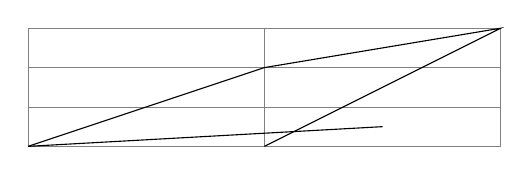
\begin{tikzpicture}[xscale=3, yscale=0.5]
\draw[help lines] (0,0) grid (2, 3);
\draw (0,0) -- (1,2) -- (2,3) -- (1,0);
\draw (0,0) -- (1.5, 0.5);
\end{tikzpicture}
\caption{tike lines.}
\end{figure}


\subsection{Arrows}
Arrows.
\begin{figure}[htbp]
\begin{tikzpicture}
\draw [->] (0,-0.8) -- (2,-0.8);
\draw [<-] (0, -0.5) -- (2, -0.5);
\draw [|->] (0,-1) -- (2,-1);
\draw [<->] (0,2) -- (0,0) -- (3,0);
\end{tikzpicture}
\caption{Arrow tutorial.}
\end{figure}

\subsection{Line Thickness}
Change line thickness.
\begin{figure}[htbp]

\begin{tikzpicture}[scale=3]
\draw [ultra thick] (0,1) -- (2,1);
\draw [thick] (0, 0.5) -- (2, 0.5);
\draw [thick] (0, 0.5) -- (2,0.5);
\draw [thin] (0,0) -- (2,0);
\end{tikzpicture}
\caption{Different line widths.}
\end{figure}

Add help lines.
\begin{figure}[htbp]
\begin{tikzpicture}[scale=3]
\draw [<->] (0,2) -- (0,0) -- (4,0);
\draw [thick] (0, 1.5) -- (3,0);
\draw [ultra thick] (0,0) -- (2,2);
\draw [help lines] (1,0) -- (1,1) -- (0,1); % help lines are in fine gray color
\end{tikzpicture}
\caption{Add gray helper lines.}
\end{figure}

Customized line width:
\begin{figure}[htbp]

\begin{tikzpicture}[scale=2]
\draw [line width=12] (0,0) -- (2,0);
\draw [line width=0.2cm] (4, 0.75) -- (5, 0.25);
\end{tikzpicture}
\caption{Customized line width.}
\end{figure}

\clearpage
\subsection{Dash \& dots}
Making dotted and dashed lines:
\begin{figure}[htbp]
\begin{tikzpicture}[scale=3]
\draw [dashed, ultra thick] (0,1) -- (2,1);
\draw [dashed] (0, 0.5) -- (2, 0.5);
\draw [dotted] (0,0) -- (2,0);
\end{tikzpicture}
\caption{Dash and dotted lines}
\end{figure}


\subsection{Colors}
Add colors:
\begin{figure}[htbp]

\begin{tikzpicture}[scale=3]
\draw [gray, line width=10] (0,1) -- (2,1);
\draw [red, line width=10] (0, 0.5) -- (2, 0.5);
\draw [blue, line width=20] (0,0) -- (2, 0);
\draw [cyan, line width=10] (0,-0.5) -- (2, -0.5);
\draw [orange, line width=10] (0, -1) -- (2, -1);
\draw [lime, line width = 10] (0, -1.5) -- (2, -1.5);
\end{tikzpicture}
\caption{Add colors.}
\end{figure}


I can also inline the tikz picture like this: 
\begin{tikzpicture} \draw [yellow, line width=6] (0,0) -- (0.5,0); \end{tikzpicture}. Cool! Right?



\section{Curves}
\subsection{Simple shapes}
Simple shapes:
\begin{figure}[htbp]

\begin{tikzpicture}
\draw [blue] (0,0) rectangle (1.5, 1);
\draw [red, ultra thick] (3, 0.5) circle [radius=0.5];
\draw [gray, line width = 10] (6,0) arc [radius=1, start angle=45, end angle=120];
\end{tikzpicture}
\caption{Simple shapes.}
\end{figure}

Smooth turns:
\begin{figure}[htbp]

\begin{tikzpicture}
\draw [<->, rounded corners, line width=5, purple] (0,2) -- (0, 0) -- (3,0);
\end{tikzpicture}
\caption{Smooth path.}
\end{figure}

Using Mathematica to pre-compute path points:
\begin{figure}[htbp]
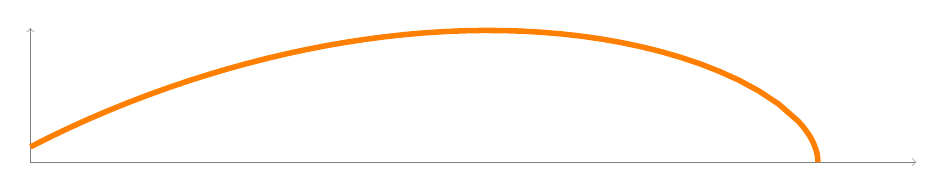
\begin{tikzpicture}[xscale=25,yscale=5]
\draw [<->, help lines] (0.6,1.34) -- (0.6,1) -- (1.05,1);
\draw[orange, line width=2] (0.6, 1.0385) --
(0.61, 1.06372) -- (0.62, 1.08756) -- (0.63, 1.11012) -- (0.64,
1.13147) -- (0.65, 1.15166) -- (0.66, 1.17074) -- (0.67, 1.18874) -- (0.68,
1.20568) -- (0.69, 1.22157) -- (0.7, 1.23643) -- (0.71, 1.25026) -- (0.72,
1.26307) -- (0.73, 1.27486) -- (0.74, 1.28561) -- (0.75, 1.29534) -- (0.76,
1.30402) -- (0.77, 1.31165) -- (0.78, 1.31821) -- (0.79, 1.32369) -- (0.8,
1.32806) -- (0.81, 1.33131) -- (0.82, 1.3334) -- (0.83, 1.33431) -- (0.84,
1.334) -- (0.85, 1.33244) -- (0.86, 1.32956) -- (0.87, 1.32533) -- (0.88,
1.31966) -- (0.89, 1.3125) -- (0.9, 1.30373) -- (0.91, 1.29325) -- (0.92,
1.2809) -- (0.93, 1.26649) -- (0.94, 1.24976) -- (0.95, 1.23032) -- (0.96,
1.2076) -- (0.97, 1.18065) -- (0.98, 1.14763) -- (0.99, 1.1038) -- (0.991,
1.09836) -- (0.992, 1.09261) -- (0.993, 1.0865) -- (0.994, 1.07994) -- (0.995,
1.07282) -- (0.996, 1.06497) -- (0.997, 1.0561) -- (0.998, 1.04563) -- (0.999,
1.03209) -- (0.9991, 1.03042) -- (0.9992, 1.02866) -- (0.9993,
1.02679) -- (0.9994, 1.02478) -- (0.9995, 1.0226) -- (0.9996, 1.02019) -- (0.9997,
1.01747) -- (0.9998, 1.01424) -- (0.9999, 1.01005) -- (0.9999,
1.01005) -- (0.99991, 1.00953) -- (0.99992, 1.00898) -- (0.99993,
1.0084) -- (0.99994, 1.00778) -- (0.99995, 1.0071) -- (0.99996,
1.00634) -- (0.99997, 1.00549) -- (0.99998, 1.00448) -- (0.99999, 1.00317) -- (1,
1) ;
\end{tikzpicture}
\caption{Using Mathematica to pre-compute points.}
\end{figure}

An easier way to plot curves:
\begin{figure}[htbp]
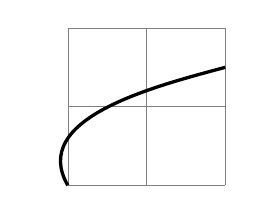
\begin{tikzpicture}
\draw[help lines] (0,0) grid (2, 2);
\draw[very thick] (0,0) to [out=120,in=195] (2, 1.5);
\end{tikzpicture}
\caption{Easier way to plot curves.}
\end{figure}

A snake arrow:
\begin{figure}[htbp]
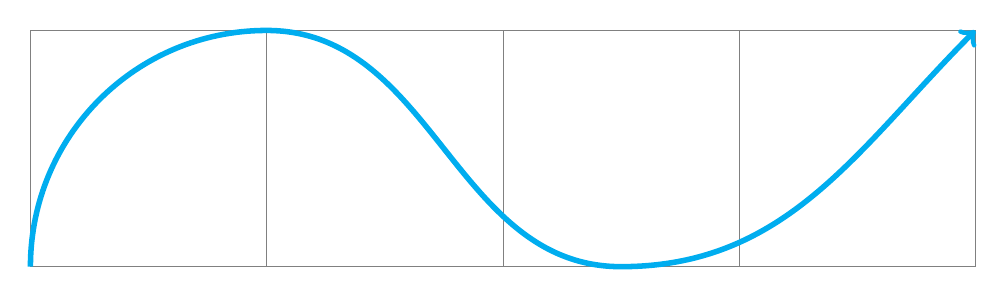
\begin{tikzpicture}[scale=3]
\draw [help lines] (0,0) grid (4,1);
\draw[->, line width=2,cyan] (0,0) to [out=90, in=180] (1,1)
   to [out=0,in=180] (2.5, 0) to [out=0, in=-135] (4,1);
\end{tikzpicture}
\caption{Snake arrow.}
\end{figure}







\end{document}  

